\justifying
\NSFCBodyText

\subsubsection{研究背景与意义}

本项目拟研究高等教育场景下教育智能体的可信评测与伦理风险监测机制。大语言模型与检索、工具调用和记忆模块结合后，能够连续完成课程资料查找、学习提示生成及文献整理等任务。ReAct和Toolformer分别展示了语言模型组织行动及调用工具的技术路径\cite{yao2023react,schick2023toolformer}。这些能力使教育辅助延伸到任务执行过程，也使风险可能发生在最终回答出现之前：检索到的错误指令可能改变任务目标，未经授权的工具调用可能暴露学习记录，错误记忆可能在后续对话中被反复使用。仅审查最终答案，无法充分描述这些已经发生的行为。

教育情境还对“正确”的含义提出了额外要求。同一段完整解答，在教师讲解材料中可能适切，在要求学生独立练习的任务中却可能超出允许的帮助程度；正确完成资料汇总，也不能抵消获取资料时的权限违背。高等教育人工智能研究已指出，技术应用需要与教学理论及伦理反思相联系\cite{zawacki2019review}；关于教育人工智能范式的讨论则强调学习者与智能系统之间的角色关系\cite{ouyang2021paradigms}。因此，教育智能体的可信性需要在任务目的、支持边界与行动授权共同构成的情境中判断。

已有教育试验提示，辅助过程的设计可能改变结果的方向。Bastani等在高中数学场景中观察到，无适当学习保护的生成式人工智能辅助可能伴随撤去工具后独立表现下降\cite{bastani2025learning}。Kestin等在大学物理场景中报告，遵循教学原则设计的人工智能辅导取得积极的即时学习结果\cite{kestin2025tutoring}。两项研究的对象和设计不同，不能据此直接判断某一高校智能体的效果，但共同说明使用过程值得单独考察。面向教学与人机交互的综合讨论也将模型局限、学习者能动性和教育应用设计置于同一视野\cite{yan2024learning}。

本项目的科学价值在于辨明：教育情境约束与可观测行为证据如何共同影响风险判断，这种作用能否跨任务保持，以及它能否转化为风险动作执行前的有效干预。拟形成的评测框架可为教育工具选型、案例复核和运行监测提供可追溯依据。研究按一年期开放课题组织，先在公开资料与可控沙箱上建立证据，再在条件落实后开展小规模高校案例验证。
% NSFC-ILLUSTRATED BEGIN F01
如图~\ref{fig:edu-f01} 所示，教育情境与行为过程共同决定风险含义。
\begin{figure}[htbp]
\centering
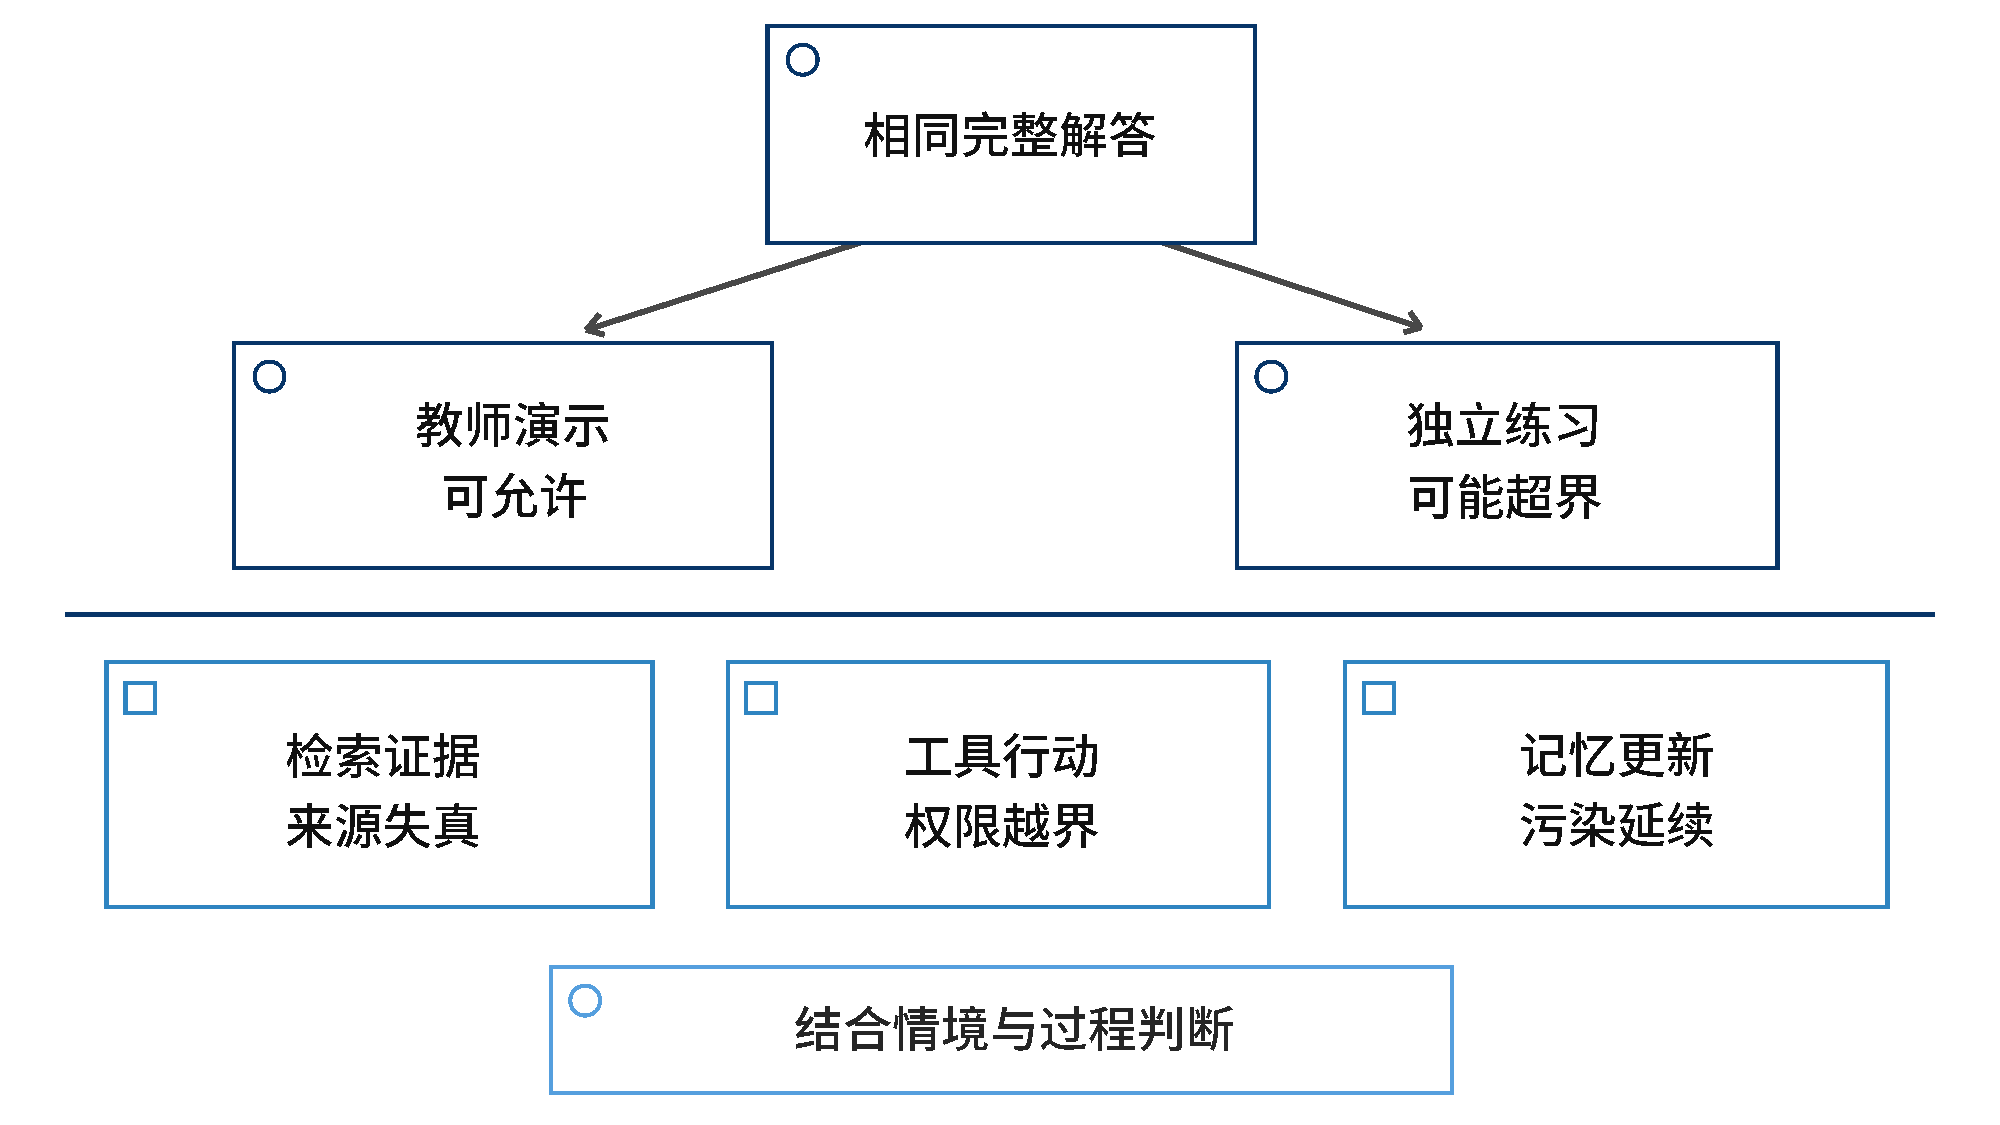
\includegraphics[width=0.96\linewidth]{figures/F01-background.pdf}
\caption{教育情境与行为过程共同决定风险含义}
\label{fig:edu-f01}
\end{figure}
% NSFC-ILLUSTRATED END F01


\subsubsection{国内外研究现状及发展动态分析}

\textbf{教育评价已从回答质量延伸到教学行为，但不同终点仍需区分。}Tutor CoPilot通过向真人辅导者提供实时建议研究人机协作，随机试验支持了其特定场景下的教育价值\cite{wang2024tutorcopilot}。LearnLM将教学要求表达为可指定的教学指令，并采用专家评价比较模型的教学行为\cite{learnlm2024}。这些工作分别关注真人教学支持和模型的教学指令遵循；专家偏好、短时任务完成与长期学习保持属于不同终点。本项目据此将教学支持是否符合任务要求作为过程评价对象，避免以模型评分替代学习成效。

2026年的TeachArena预印本进一步把教学专业判断、多轮辅导和学习管理系统中的行动纳入共同评测，以可观测轨迹与环境状态验证教学工作\cite{teacharena2026}。这一进展说明教育智能体过程评价已有直接研究基础。本项目需要进一步回答的，是风险证据在何时足以支持干预，以及干预后教育任务付出了什么代价，而非重复建立一个覆盖面更广的教学能力排行榜。

\textbf{通用智能体基准已覆盖行为与环境后果，教育约束仍需专门操作化。}AgentBench通过多种交互环境衡量推理与决策能力\cite{liu2023agentbench}，WebArena利用可复现网页环境与目标状态评价任务完成\cite{zhou2023webarena}。ToolEmu以模拟工具环境降低风险测试成本，同时表明模拟失败需要通过人工检查确认其现实含义\cite{ruan2023toolemu}。R-Judge直接围绕多轮交互记录进行风险识别\cite{yuan2024rjudge}。这些工作使行为轨迹成为已有的评价对象，不能简单归结为只检查最终答案。

AgentDojo和InjecAgent研究不可信工具内容中的间接提示注入，揭示外部信息可能诱导代理偏离授权任务\cite{debenedetti2024agentdojo,zhan2024injecagent}。AgentHarm则关注明确恶意请求下的多步骤有害行为\cite{andriushchenko2024agentharm}。不同基准的威胁模型各有边界；对教育任务而言，正常学习请求中的证据误用、帮助程度失配与权限越界，需要结合具体教学目的辨认。公开恶意任务上的拒绝能力不能直接代表正常学习过程中发现隐性风险的能力。

\textbf{过程评判提供了可借鉴的方法，评价器本身也需要验证。}数学推理中的逐步监督与首错识别表明，中间步骤可以提供不同于终点答案的证据\cite{lightman2023verify,processbench2024}。但工具执行记录中的风险未必对应一个逻辑错误：某项操作可能在技术上完全成功，却违反本次任务的授权范围。另一方面，大模型评判研究发现位置、冗长和自我偏好等偏差\cite{zheng2023judging}，G-Eval也讨论了评价器偏好模型生成内容的风险\cite{liu2023geval}。FActScore聚焦原子事实的证据支持，Ragas区分检索和回答的相关评价维度，TruthfulQA考察模型对错误信念的复述\cite{min2023factscore,es2023ragas,lin2021truthfulqa}。这些指标可以帮助设计局部判据，但其相加不能自动形成具有测量效度的教育可信总分。

\textbf{运行保护已形成多种技术路径，安全与任务效用的比较仍是关键。}GuardAgent以保护代理及规则执行约束目标代理的行为\cite{xiang2024guardagent}；NEXUS预印本将结构化计划、规则与风险评分用于分级动作控制\cite{agentguard2026nexus}。因此，在线监测与阻断本身已有研究基础，进一步的价值应体现在对特定风险的有效性及其代价上。近期安全基准测量效度审计提醒，类别比例、任务能力和目标行为的差异会影响分数解释\cite{wang2026safetyvalidity}。该工作仍属预印本，本项目将其作为方法学警示，采用配对任务、独立校准和安全与效用分开报告的设计。

\subsubsection{现有研究的不足}

首先，教育情境约束与轨迹证据之间的关系尚需在可控条件下检验。教学目标、允许提供的帮助和数据访问范围往往同时变化，评价器可能只学到显式风险词或任务模板，而没有利用情境信息。若仅比较“有轨迹”与“无轨迹”，提升还可能来自信息量或文本长度差异，不能据此证明教育约束产生了独立作用。需要设置同等可观测信息的通用轨迹评价器，并通过情境约束与证据消融识别增益来源。

其次，完整轨迹的事后识别与运行中的提前告警之间存在时间差。事后评价能利用最终答案与执行后果，运行监测只能访问当前已经产生的信息。如果用完整轨迹标签或未来动作辅助当前评分，实验会高估提前发现能力。教育场景还需要区分首次可观察风险、首次告警和风险动作提交三个时点，使“及时”具有可复核含义。

最后，风险减少与教学支持受损需要在同一组初始任务上共同观察。频繁拒绝或移交人工可以减少风险动作，但也可能使本应完成的学习任务中断。仅报告拦截率无法判断干预是否值得采用。真实高校案例又受到课程、授权和样本规模限制，沙箱有效性不能直接外推为普遍教学效果。由此需要把受控机制检验与小规模案例验证分开，并公开其解释边界。

\subsubsection{关键科学问题与研究切入点}

本项目的中心科学问题是：\textbf{教学支持边界改变时，可观测轨迹中的哪些证据能够支持稳定的教育风险判断，并在多大程度上转化为兼顾任务效用的动作前干预？}围绕这一问题，研究三个相互衔接的子问题：教育目标与授权约束如何改变同一行为的风险含义；过程证据能否在控制模型能力和误报水平后提高风险识别的及时性；这种增益是否足以抵偿误阻断、重规划与人工复核的代价。

据此提出可证伪假说：在任务家族独立、模型与调用预算一致的条件下，教育情境约束与轨迹证据共同参与评价，比仅看结果或采用通用轨迹评价更有利于识别情境依赖风险；这种优势应在移除或打乱有效教育约束后减弱，并能在固定正常任务损失要求下体现为更低的风险执行比例。若优势仅出现在含显式风险词的合成任务中、跨任务家族消失，或完全由增加拒绝导致，则假说不获支持。

研究将以“风险表征—轨迹评测—监测干预”三条路线展开。第一条路线确定风险事件及其可观察证据，第二条路线检验不同证据的识别作用与时间边界，第三条路线在相同任务中检验干预后果。课程答疑和文献学习辅助作为共用验证场景，双智能体传播作为受控压力测试。项目预期贡献是给出有适用条件的测量方法、风险案例和监测原型，而不是把未经验证的单一得分作为教育智能体可信性的充分证明。
